\chapter{Conclusions and outlook}
\label{chap:conclusions}
In this thesis analyses of proton-proton collisions recorded by the \ac{CMS} detector during
Run 1 and Run 2 of the \ac{LHC} have been presented. The focus of these analyses
is the search for \ac{BSM} Higgs bosons with tau leptons in the final state.

The search for a heavy Higgs boson decaying to a final state of $\Pbottom\Pbottom\Pgt\Pgt$ via two
$125\,\GeV$ Higgs bosons was performed using $19.7\,\invfb$ of data collected at a
centre-of mass energy of $8\,\TeV$ during the 2012 \ac{LHC} data-taking period. Such a final
state can access areas of the \ac{MSSM} parameter space not easily accessible via other channels.
To separate more signal-like and more background-like events, a categorisation based on the number of 
b-tagged jets is used. To further increase the sensitivity to the signal, cuts on the di-tau and di-jet
mass in a window around $125\,\GeV$ are used in combination with a kinematic fitting technique for
the reconstruction of the four-body mass.
The resulting mass variable provides good separation between the signal and the dominant
\ttbar background, and is thus used as the variable for signal extraction. 
The results of this search are upper limits on production cross section times branching 
ratio, in a mass range of $260<m_{\PHiggs}<350\,\GeV$. A combination with a search for \AtoZhtolltautau
yields exclusion in the lowest \tanb~region of the low-\tanb~\ac{MSSM} scenario, as well
as several areas of the \cosba-\tanb~plane in a \ac{2HDM} scenario \cite{CMS-HIG-14-034}.

Searches for heavy neutral Higgs bosons decaying into pairs of tau leptons were performed
using $2.3\,\invfb$ of data recorded during the 2015
data-taking period of the \ac{LHC}, and using $12.9\,\invfb$ of 
data recorded during the first half of the 2016 data-taking period. The 
branching ratio of heavy neutral Higgs bosons into di-tau pairs is enhanced at high \tanb~in the \ac{MSSM},
making this one of the most sensitive search channels for such particles. Both analyses use a categorisation 
based on the presence of b-tagged jets to separate
the gluon fusion and b-associated Higgs boson production modes in the \ac{MSSM}. 
The hadronic tau isolation working point and the topological selection on 
the transverse mass between the electron or muon and the missing transverse energy are chosen to optimise the search sensitivity for signal
masses of around $1\,\TeV$.
The sensitivity is maximised by using the total transverse mass for signal extraction. This variable, which is 
the combination of the transverse
mass between the two legs of the di-tau candidate and the transverse masses between each of the legs
of the di-tau candidate and the missing transverse energy,
separates the dominant backgrounds
and the high-mass signal well.
No significant excess is observed in these searches, and so 
these analyses set limits on the production cross section times branching ratio of both the
gluon fusion and b-associated production processes. The results are also
interpreted in \ac{MSSM} benchmark scenarios, where the analyses exclude large areas
of the \mA-\tanb~plane, with significant improvement with respect to the most sensitive
results obtained in Run 1 \cite{CMS-PAS-HIG-16-006,CMS-PAS-HIG-16-037}. A combination of the 2015 and 2016 analyses is also
performed. This combination improves on the results of the 2016 analysis alone, thus
setting the most stringent limits on $\PHiggsps/\PHiggs$ production to date.

As more data are collected during the remainder of Run 2, and in the 
future, searches for \ac{MSSM} Higgs bosons in the di-tau final
state will continue. If no such Higgs bosons are found, these searches
will be able to exclude even more of the \mA-\tanb~plane in specific
\ac{MSSM} benchmark scenarios, although not all of the \mA-\tanb~plane
will become accessible. A projection of the results of the 2015 \ac{MSSM}
analysis to integrated luminosities of $300\,\invfb$ and $3000\,\invfb$ \cite{HTT-projection} is
shown in figure \ref{fig:mssm_projection_fig}. Even with an integrated luminosity of
$3000\,\invfb$ it is not possible to exclude the full \mA-\tanb~plane of this scenario,
as the branching ratio of $\PHiggsps/\PHiggs$ into di-tau pairs 
is very low in the high-\mA~and low-\tanb~corner. This region can be accessed 
via searches for the $\PHiggsps/\PHiggs \rightarrow \Ptop\APtop$ decay, which
has an enhanced branching ratio in this region. To fully cover this
parameter space it will therefore start to become more and more
important to combine searches for heavy Higgs bosons in different final states.
Doing this will give the best sensitivity to possible
heavy Higgs bosons, or in the absence of these particles exclusion
of the scenarios that predict them.

\begin{figure}[h!]
\begin{center}
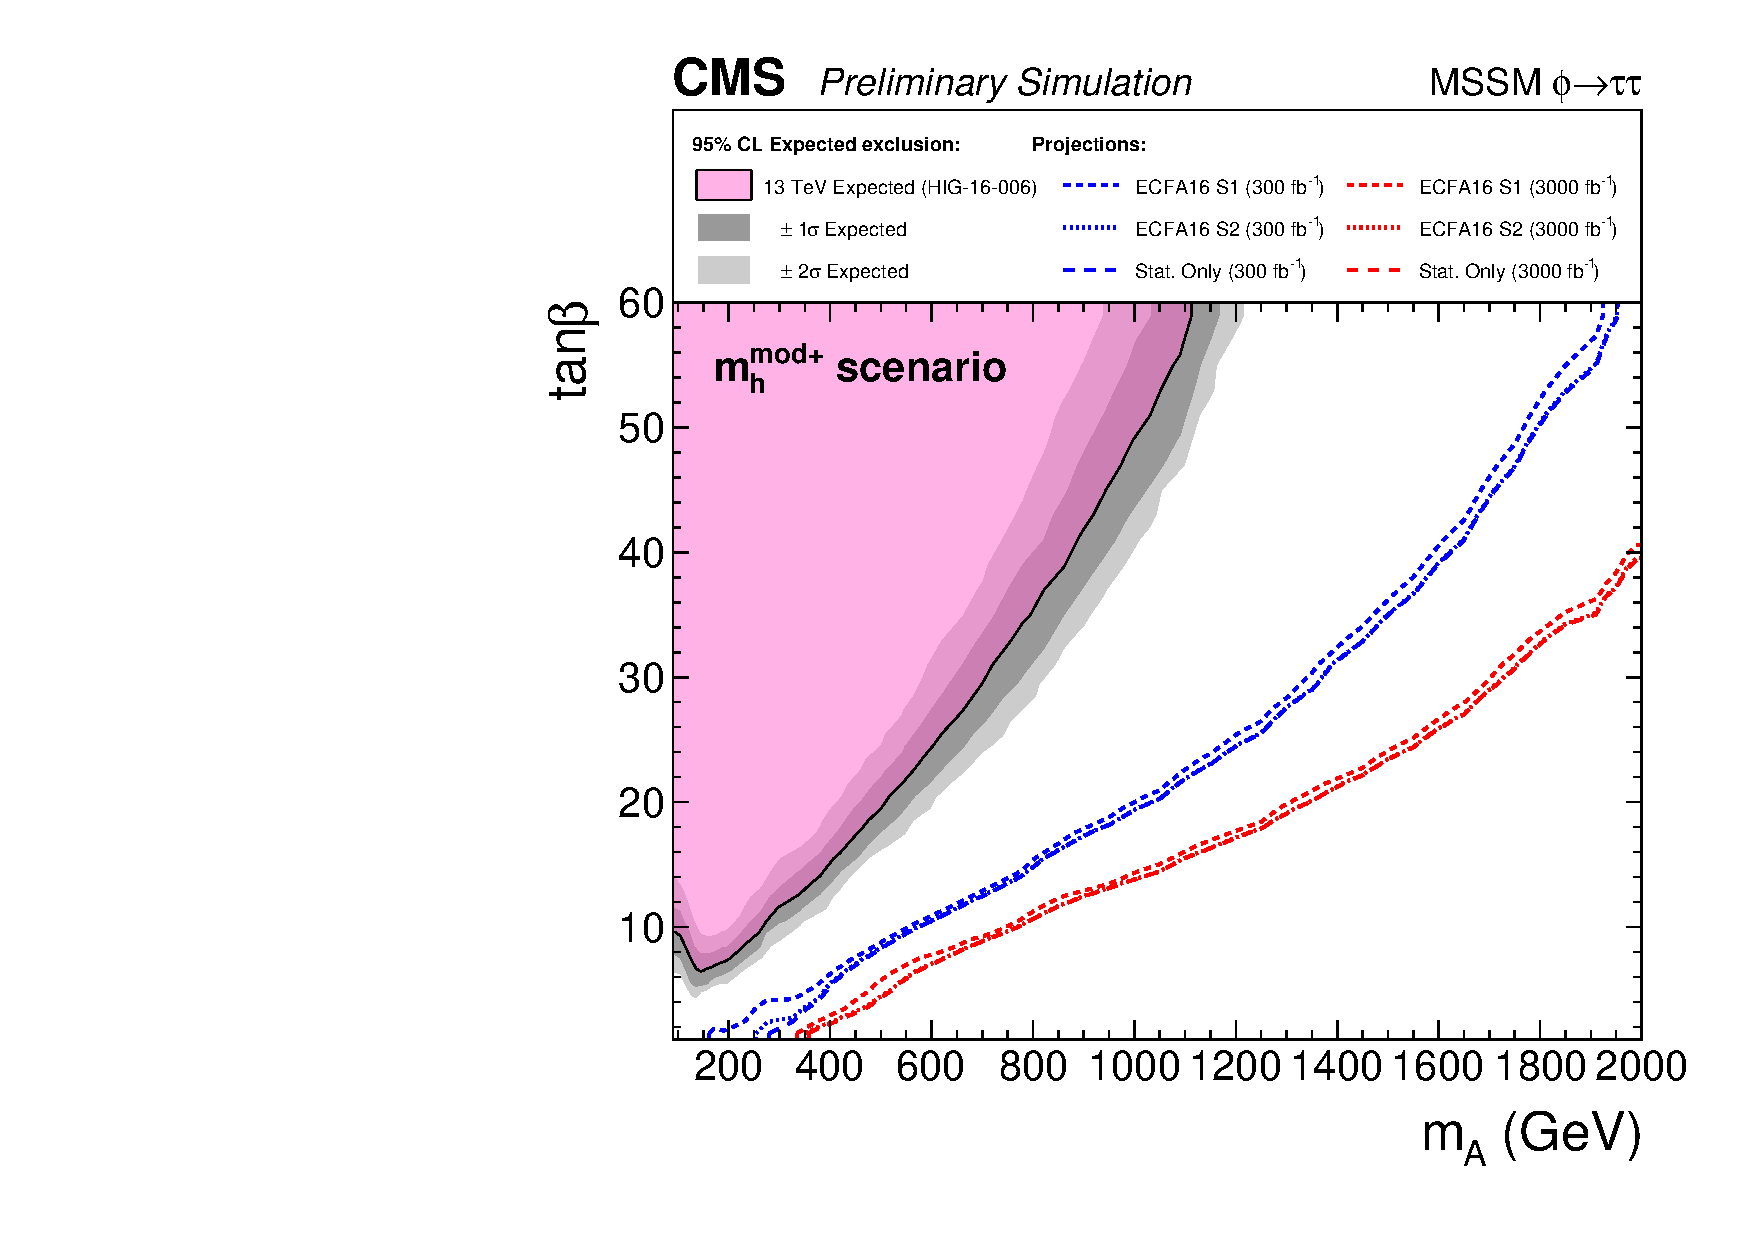
\includegraphics[width=0.7\textwidth]{./Conclusion/Figures/scenario_comp2.pdf}
\end{center}
\caption[The expected exclusion in the $m_{\PHiggslight}^{\text{mod+}}$ scenario
at the 95\% CL of the 2015 MSSM analysis, projected to integrated luminosities of $300$ and $3000\,\invfb$.]{The expected exclusion in the $m_{\PHiggslight}^{\text{mod+}}$ scenario
 at the 95\% CL of the 2015 MSSM analysis (pink)
projected to integrated luminosities of $300\,\invfb$ (blue) and $3000\,\invfb$ (red)
under several assumptions of how the systematic uncertainties scale. In scenario ``S1''
all systematic uncertainties are kept constant with integrated luminosity, while in scenario ``S2'' 
the theoretial uncertainties are scaled down by a factor $\frac{1}{2}$ and experimental
systematic uncertainties scale down by the square root of the integrated luminosity until they reach
a lower limit. In the ``Stat. Only'' scenario all systematic uncertainties are neglected. Even with an integrated 
luminosity of $3000\,\invfb$ it is not possible to exclude the entire \mA-\tanb~plane
in this \ac{MSSM} benchmark scenario using this analysis alone \cite{HTT-projection}.}
\label{fig:mssm_projection_fig}
\end{figure}

